%-------
% Gayatri Belapurkar's resume.
%-------

%-------
% Basic configurations for the document. This resume makes use of the res.cls template, a copy of which can be found 
% on https://rpi.edu/dept/arc/training/latex/resumes/ 
%-------
\documentclass[margin]{res}
\textwidth=5.2in 
            		 
% Use pdf, png, jpg, or eps§ with pdflatex; use eps in DVI mode
\usepackage{graphicx}														

\begin{document}

%---
% Defining new command for superscript usage
%---
\newcommand{\ts}{\textsuperscript} 

%----
% Basic details 
%----
\name{Gayatri Vyankatesh Belapurkar\\[13pt]}
\address{{\bf Address} \\91-A, Kamgar Nagar \\ Kurla East \\ Mumbai-400024}
\address{{\bf Contact Details} \\Mob: +91-9920697529 \\ Email: gayatri.belapurkar5@gmail.com}

\begin{resume}

%----
% Photo
%----
\begin{figure}[h!]
    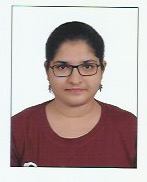
\includegraphics[scale=0.5]{Photo_gayatri.jpeg}
\end{figure}

%----
% Section: Objective
%----
\section{Career Objective}
Seeking to work as a software development engineer to solve real world problems using Machine Learning, Artificial Intelligence and Data Science.

%----
% Section: Education
%----
\section{Education}
\begin{table}[h!]
  \begin{tabular}{p{0.5cm}|p{4cm}|p{3.5cm}|p{2cm}|p{1.5cm}|p{1.6cm}}
    \textbf{Sr.} & \textbf{Degree} & \textbf{College} & \textbf{University} & \textbf{Passing Year} & \textbf{Pass Percentage} \\
    \hline
    1. & B.E., Information Technology. & Vivekanand Education Society's Institute of Technology. & University of Mumbai. & 2020 & 8.94\\
    2. & XII\ts{th} Higher Secondary Certificate. & Swami Vivekanand Junior College. & Maharashtra State Board. & 2016 & 84.77\%\\
    3. & X\ts{th }C.B.S.E. & Atomic Energy Central School-6. & Central Board of Secondary Education. & 2012 &  97.6\%\\
    \end{tabular}
\end{table}

%----
% Section: Projects
%----
\section{Projects}
\begin{enumerate}
  \item {\bf Smart Subsidy System using blockchain}
  
  This project was my entry for Smart India Hackathon 2019 for creating a digital subsidy system using blockchain technology to ensure that the subsidies are received by the true beneficiaries. This project reduced the tracks the application at every stage, reduces the time delays, reduces fraud involved in subsidy distribution and ensures that the records are immutable. As a part of project implementation, I used Ionic framework for hybrid mobile application development and  Solidity for blockchain.
  \item {\bf IoT based Street Quality Identification}
  
  This project is an IoT based solution for measuring of Street Quality by identifying and mapping potholes on the street. I worked in a team of 4 for implementing the project and used a 6 axes accelerometer along with NodeMCU for measuring the vibrations, and GPS module neo6mv2 with Raspberry Pi for mapping the these vibrations to location co-ordinates. The data from this setup was sent to Google Firebase and we used Smooth Z-score algorithm which gave a dynamic threshold which was used for identification of pothole from the data collected from the accelerometer. The web interface, built using Django (Python), displayed the details of the potholes and street quality on a color coded map. This was a completely wireless and a pluggable setup which made it easy to plug and play on any vehicle.
  \item {\bf IoT based detection of public toilet usage and incentivization}
  
  This project was aimed towards detection of usage of public toilets and provide incentives to individuals who use them, thus developing a good hygiene habit. I worked in a team of 4 for implementing this project. The system used a proximity sensor to detect the occupancy of a toilet stall/booth, a turbidity sensor which detected the actual human waste in the toilet and a finger print sensor to identify an individual. These sensors were connected to Raspberry Pi which sent data to Google Firebase and incentives were provided to individuals based on parameters such as consistent daily usage of these public toilets. This data was also available through a mobile application developed using React Native. 
   \item {\bf Asset Management System}
  
  This project was aimed towards solving the problem of laboratory supplies management in colleges by facilitating allocation, purchases and inter-departmental transfers of assets such as monitors, processors, project supplies, etc. I worked in a team of 5 to implement this project using Laravel framework for PHP and SQL for database.
  \item {\bf Blockchain based connectivity for content providers and users for education}
  
  This project was based on the idea of connecting tutors to students using Blockchain for keeping the records related to users and content providers safe and secure and generate certificates which can be stored securely. The implementation of this project was mainly in Laravel framework for PHP and used Python for prototyping Blockchain. 
\end{enumerate}

  %----
  % Internship
  %----
  \section{Internships}
  \begin{itemize}
    \item {\bf Software Development Internship},  AppStack \hfill Jun 2018 - Oct 2018
    
    Worked as an intern with AppStack, a Canada based startup, for Android and iOS application development. My primary project was development of a mobile application which allowed users to post images of photos of food dishes along with its recipes. I was responsible for designing the software architecture of the application, the end to end user experience, implementation and testing of the project. During course of the internship, I used React Native for mobile application development and Google Firebase for database.
    \item {\bf Winter Internship}, VESIT \hfill Dec 2017 - Jan 2018
    
    Worked as an intern on developing staff attendance module in VESIT Content Management System. During the internship, I  focused primarily on developing attendance synchronization and data transfer of records between the biometric attendance module and server using Java for backend and MySQL for database.
 \end{itemize}
 
%----
% Research Publications
%----
\section{Research Publication}
\begin{enumerate}
  \item None. 
\end{enumerate}

%----
% Technical Skills
%----
\section{Technical Skills}
\begin{itemize}
  \item Programming Languages: C, C++, Java, Python
  \item Mobile App Development using React Native and Ionic
  \item Web development using HTML, CSS, PHP, Laravel framework
  \item Data mining and database management
  \item Basics of Machine Learning
\end{itemize}

%----
% Soft Skills
%----
\section{Soft Skills}
\begin{enumerate}
  \item Team leader and team player
  \item Responsible
  \item Efficient communicator
  \item Rational and logical perspective
  \item Problem solving and conflict resolution
\end{enumerate}

%----
% Extra Curricular Activities
%----
\section{Extra Curricular Activities}
\begin{itemize}
  \item {\bf Student Chief Editor}, VESIT Connect \hfill Apr 2018 - Present
  
  Currently working as the Student Chief Editor of VESIT Connect (monthly newsletter) and of Vishwakarma (annual magazine)  of Vivekanand Education Society's Institute of Technology. 
  \item {\bf VESIT Badminton team} \hfill Sep 2018 - Present
  
  Part of the VESIT Badminton team and represented the college at various tournaments for singles and doubles. 
  \item {\bf Student Reporter}, VESIT Connect \hfill Jul 2017 - Mar 2018
  
  Worked as the Student Reporter at VESIT Connect, before heading the team as Student Chief Editor. 
  
  \item {\bf Drama event}, Utsav \hfill Mar 2018
  
  Participated and won the group drama event in Utsav, which is the annual cultural festival of VESIT.
  \item {\bf Technical Assistance Team}, Praxis \hfill Sep 2017
  
  Worked towards providing technical assistance for Praxis, which is the annual technical festival of VESIT. 
  \item {\bf Aesthetic team}, Illusions \hfill Jan 2017
  
  Competed in aesthetic front in Illusions, which is the annual cultural competition in VESIT.
\end{itemize}

%----
% Co-Curricular Activities
%----
\section{Co-Curricular Activities}
\begin{enumerate}
\item {\bf Workshop on Convolution Neural Network}, VESIT \hfill Mar 2019

Attended a workshop for Convolution Neural Network, organized in VESIT for promoting participation of women in applied data science areas. 
\item {\bf Cloudera Certification}, VESIT/Cloudera \hfill Sep 2018 - Mar 2019

Completed Cloudera certification for Big Data using Hadoop. 
\end{enumerate}

%----
% Achievements
%----
\section{Achievements}
\begin{itemize}
\item Winner of Smart India Hackathon, 2019
\item Winner in 'Best Algorithm' category in eYantra Ideas Competition, 2019
\item Semi-finalist in Project Deep Blue, 2019
\item Winner of hackathon 'VESIT Hacks' held in Praxis 2018
\item Top 25 teams in ACM Women's Hackathon. 
\item Won multiple events in VESIT cultural festival - Utsav in 2018 (2\ts{nd} in Drama, 2\ts{nd} in Rangoli, 2\ts{nd} in Paper Dressing, 3\ts{rd} in Tshirt Painting and Nail art)
\item Semi-finalist in inter-college Badminton Competition (women's doubles) in Skream, the Annual Sports Festival organized by K.J. Somaiya College.
\item Quarter-finalist in inter-college Badminton Competition (women's singles) in Skream, the Annual Sports Festival organized by K.J. Somaiya College.
\item Winner of hackathon 'VESIT Hacks' held in Praxis 2017 (Junior category)
\end{itemize}

%----
% Personal Information
%----
\section{Personal Information}
Father's Name: Vyankatesh Chandrakant Belapurkar

Mother's Name: Manisha Vyankatesh Belapurkar

Sex: Female

Date of Birth: 25/11/1998

Nationality: Indian

Marital Status: Single

%----
% Declaration
%----
\section{Declaration}
I, Gayatri Belapurkar, hereby declare that the information in this document/curriculum vitae is true as of the date given below. 

%----
% Date
%----
\section{Date}
17/04/2019

\end{resume}

\end{document}  